% ============================================================
%  Dal-i — Informe del Projecte
%  UAB · Sistemes Multimèdia 2025–2026 · Grup G4-6
%  Compilar amb:  latexmk main.tex
% ============================================================
\documentclass[11pt, a4paper]{article}

% ── url must be loaded before hyperref to pass hyphens option ─
\PassOptionsToPackage{hyphens}{url}

% ── Idioma i fonts (LuaLaTeX) ────────────────────────────────
\usepackage{fontspec}
\setmainfont{TeX Gyre Pagella}
\setsansfont{TeX Gyre Heros}[Scale=MatchLowercase]
\setmonofont{IBM Plex Mono}[Scale=MatchLowercase]
\usepackage[catalan]{babel}
\usepackage[
  protrusion=true,
  expansion=true,
  factor=1100,
  stretch=15,
  shrink=15
]{microtype}

% ── Pàgina ───────────────────────────────────────────────────
\usepackage[top=2.5cm, bottom=2.5cm, left=3cm, right=2.5cm]{geometry}
\usepackage{parskip}
\setlength{\headheight}{15pt}

% ── Capçalera i peu de pàgina ────────────────────────────────
\usepackage{fancyhdr}
\pagestyle{fancy}
\fancyhf{}
\fancyhead[L]{\small\color{gray}Dal-i — Sistema Robòtic de Dibuix Col·laboratiu}
\fancyhead[R]{\small\color{gray}Grup G4-6 · UAB SM 2025–26}
\fancyfoot[C]{\thepage}
\renewcommand{\headrulewidth}{0.4pt}

% ── Colors ───────────────────────────────────────────────────
\usepackage{xcolor}
\definecolor{dalblue}{HTML}{1A73E8}
\definecolor{lightgray}{HTML}{F5F5F5}
\definecolor{mintbg}{HTML}{F8F8F8}

% ── Gràfics ──────────────────────────────────────────────────
\usepackage{graphicx}
\usepackage{float}
\usepackage{subcaption}
\usepackage{caption}
\captionsetup{font={small,sf}, labelfont={bf,sf}}
\graphicspath{{images/}{../presentation/images/}}

% ── Maths ────────────────────────────────────────────────────
% unicode-math must come after fontspec; XITS Math is in TeXLive full
\usepackage{amsmath}
\usepackage{unicode-math}
\setmathfont{TeX Gyre Pagella Math}[Scale=MatchLowercase]

% ── TikZ ─────────────────────────────────────────────────────
\usepackage{tikz}
\usetikzlibrary{arrows.meta, positioning, calc, fit, backgrounds}
\tikzset{every node/.style={font=\sffamily}}

% ── Taules ───────────────────────────────────────────────────
\usepackage{booktabs}
\usepackage{array}
\usepackage{tabularx}
\usepackage{etoolbox}
\AtBeginEnvironment{tabular}{\sffamily}
\AtBeginEnvironment{tabularx}{\sffamily}

% ── Codi font (minted) ───────────────────────────────────────
\usepackage{minted}
\setminted{
  fontsize=\small,
  bgcolor=mintbg,
  frame=lines,
  framesep=2mm,
  linenos=true,
  breaklines=true,
  breakanywhere=true,
  breakautoindent=true,
  numbersep=5pt,
  xleftmargin=0pt,
  xrightmargin=0pt,
}
\setmintedinline{fontsize=\small, bgcolor={}}

% ── Icones ───────────────────────────────────────────────────
\usepackage{fontawesome5}

% ── Taula de continguts (sans-serif) ─────────────────────────
\usepackage{tocloft}
\renewcommand{\cfttoctitlefont}{\Large\sffamily\bfseries}
\renewcommand{\cftsecfont}{\sffamily\bfseries}
\renewcommand{\cftsecpagefont}{\sffamily}
\renewcommand{\cftsubsecfont}{\sffamily}
\renewcommand{\cftsubsecpagefont}{\sffamily}
\renewcommand{\cftsubsubsecfont}{\sffamily}
\renewcommand{\cftsubsubsecpagefont}{\sffamily}

% ── Seccions ─────────────────────────────────────────────────
\usepackage{titlesec}
\titleformat{\section}{\large\sffamily\bfseries}{{\thesection}}{0.8em}{}
\titleformat{\subsection}{\normalsize\sffamily\bfseries}{{\thesubsection}}{0.8em}{}
\titleformat{\subsubsection}{\normalsize\sffamily}{{\thesubsubsection}}{0.8em}{}

% ── Enllaços ─────────────────────────────────────────────────
\usepackage{hyperref}
\hypersetup{
  colorlinks=true,
  linkcolor=black,
  urlcolor=dalblue,
  citecolor=black,
  pdftitle={Dal-i — Informe del Projecte},
  pdfauthor={Grup G4-6, UAB Sistemes Multimedia},
}

% ── Bibliografia (biblatex + biber) ──────────────────────────
\usepackage[
  backend=biber,
  style=numeric,
  sorting=none,
  urldate=long,
  maxbibnames=99,
]{biblatex}
\addbibresource{references.bib}

% ── Cross-references (bold figures, tables, listings) ────────
% cleveref must load after hyperref
\usepackage{cleveref}
\crefformat{figure}{\textbf{Figura~#2#1#3}}
\crefformat{table}{\textbf{Taula~#2#1#3}}
\crefformat{listing}{\textbf{Codi~#2#1#3}}
\crefformat{section}{Secció~#2#1#3}

% ── DOI helper ───────────────────────────────────────────────
\newcommand{\doi}[1]{\href{https://doi.org/#1}{\textsc{doi}: #1}}

% ── Arrow for text mode (Noto Serif lacks U+2192) ────────────
\newcommand{\arw}{\ensuremath{\rightarrow}}

% ── Allow \texttt{} to break across lines ────────────────────
\usepackage[htt]{hyphenat}

% ── Inline code helpers ───────────────────────────────────────
% \code{} for short inline identifiers; \codepath{} for breakable paths
\newcommand{\code}[1]{\mintinline{text}{#1}}
\newcommand{\codepath}[1]{\path{#1}}

% ============================================================
\begin{document}

% ── Portada ──────────────────────────────────────────────────
\begin{titlepage}
  \centering\sffamily

  
\includegraphics[width=6cm]{./images/logotipuab-v1-verd.png}

  {\large Universitat Autònoma de Barcelona}\\[0.3cm]
  {\normalsize Grau en Sistemes Multimèdia · Curs 2025–2026}\\[0.2cm]
  {\normalsize Hackathon — Informe del Projecte}

  \vspace{0.5cm}

  {\fontsize{42}{48}\selectfont\textbf{\color{dalblue}Dal-i}}\\[0.5cm]
  {\Large Sistema Robòtic de Dibuix Col·laboratiu}\\[0.3cm]
  \rule{0.6\linewidth}{0.8pt}\\[0.3cm]
  {\normalsize\color{gray} Generació automàtica de trajectòries per a braç robòtic\\
  mitjançant visió per computador i intel·ligència artificial generativa}

  \vspace{0.6cm}
  
  
\includegraphics[width=5cm]{../presentation/images/logo.jpeg}

  \vspace{0.6cm}

  {\large\textbf{Grup G4-6}}

  \vspace{1.2cm}

  \begin{tabular}{@{}lc@{}}
    \toprule
    \textbf{Nom i Cognoms}    & \textbf{NIU} \\
    \midrule
    David Madueño Noguer      & 1526933 \\[4pt]
    Moisés Sánchez Pin        & 1603611 \\[4pt]
    Xavier Cañada Escalona    & 1708948 \\[4pt]
    Lorenzo Payaro Robles     & 1731940 \\
    \bottomrule
  \end{tabular}

  \vfill
  {\normalsize Juny 2026}
\end{titlepage}

% ── Taula de continguts ───────────────────────────────────────
\tableofcontents
\newpage

% ── Seccions ─────────────────────────────────────────────────
\section{Introducció}

\subsection{Context}

Aquest projecte s'ha desenvolupat en el marc del \textit{hackathon} de l'assignatura de Sistemes Multimèdia del Grau en Sistemes Multimèdia de la Universitat Autònoma de Barcelona, durant el curs 2025--2026. L'objectiu del hackathon és dissenyar i implementar un sistema complet que integri múltiples tecnologies multimèdia i de computació al núvol en un termini limitat.

El projecte \textbf{Dal-i} —nom que fa referència a l'artista Salvador Dalí i al model d'IA generativa DALL-E— és un sistema que permet a qualsevol usuari crear dibuixos artístics a través d'un braç robòtic, sense necessitat de cap habilitat artística prèvia. El sistema accepta una imatge d'entrada i un estil artístic (introduïts per veu, text o selecció), processa la imatge mitjançant tècniques de visió per computador, i genera les coordenades de trajectòria que el robot ha de seguir per reproduir el dibuix.

\subsection{Motivació}

La motivació principal del projecte és construir un pont entre tres àmbits tecnològics que rarament es combinen en un sol sistema educatiu:

\begin{itemize}
  \item \textbf{Intel·ligència artificial generativa}: ús de models de difusió i transformadors per generar o transferir estils artístics.
  \item \textbf{Visió per computador clàssica}: detecció de contorns, extracció de característiques i optimització de trajectòries per a robòtica.
  \item \textbf{Arquitectura cloud-native}: desplegament escalable i de baix cost mitjançant Google Cloud Platform, amb separació de responsabilitats en microserveis.
\end{itemize}

A més, l'addició de suport multilingüe (10 idiomes) i d'entrada per veu reflecteix l'interès del grup per fer el sistema accessible a usuaris de qualsevol llengua i entorn.

\subsection{Objectius}

Els objectius principals del projecte són:

\begin{enumerate}
  \item Implementar un \textit{pipeline} complet de processament d'imatges que converteixi qualsevol fotografia en coordenades de trajectòria per a un braç robòtic SCARA.
  \item Desplegar el sistema sobre una arquitectura \textit{cloud-native} escalable, fent ús de Cloud Run i Cloud Functions de Google Cloud Platform.
  \item Oferir múltiples modalitats d'entrada: selecció d'estil per text, per veu i per botons de selecció ràpida.
  \item Integrar IA generativa (Gemini 2.5 Flash) per a la transferència d'estil visual en un mode avançat opcional.
  \item Donar suport multilingüe automàtic per permetre l'ús del sistema en 10 idiomes.
  \item Proporcionar una experiència d'usuari fluida amb historial persistent per sessió, paginació i esborrat en cascada.
\end{enumerate}

\subsection{Estructura de l'informe}

La resta d'aquest document s'organitza de la manera següent. La secció~\ref{sec:descripcio} descriu l'aplicació des del punt de vista de l'usuari. La secció~\ref{sec:arquitectura} detalla l'arquitectura del sistema. La secció~\ref{sec:desenvolupament} explica el procés de desenvolupament per fases. La secció~\ref{sec:tecnologies} llista les tecnologies utilitzades. La secció~\ref{sec:problemes} recull els problemes trobats i les solucions adoptades. La secció~\ref{sec:resultats} presenta els resultats obtinguts. Finalment, la secció~\ref{sec:conclusions} recull les conclusions i el treball futur.

\section{Descripció de l'Aplicació}
\label{sec:descripcio}

\subsection{Visió general}

Dal-i és una aplicació web que permet a l'usuari transformar qualsevol imatge en un dibuix artístic executat per un braç robòtic. El sistema actua com a intermediari entre la creativitat de l'usuari i la precisió mecànica del robot: l'usuari tria una imatge i un estil artístic, i el sistema calcula automàticament les trajectòries que el robot ha de seguir per reproduir el dibuix sobre paper.

\subsection{Flux d'ús}

El flux d'ús típic de l'aplicació és el següent:

\begin{enumerate}
  \item L'usuari accedeix a la interfície web i selecciona una imatge d'entrada (fotografia, il·lustració, etc.).
  \item L'usuari tria un estil artístic mitjançant una de les tres modalitats disponibles:
    \begin{itemize}
      \item \textbf{Selecció ràpida}: botons predefinits (Picasso, Van Gogh, Monet, Manga, etc.).
      \item \textbf{Text}: l'usuari escriu una instrucció en qualsevol dels 10 idiomes suportats.
      \item \textbf{Veu}: l'usuari grava un comandament de veu; el sistema transcriu~\cite{stt} i extreu l'estil automàticament.
    \end{itemize}
  \item Opcionalment, l'usuari pot activar el \textbf{Mode Avançat (IA Generativa)}, que usa Gemini 2.5 Flash~\cite{vertexai} per aplicar la transformació visual a la imatge abans de la detecció de contorns.
  \item El sistema processa la imatge i retorna:
    \begin{itemize}
      \item Les \textbf{coordenades} de trajectòria per al robot (llista de punts \texttt{\{x, y\}}).
      \item Una \textbf{previsualització SVG} dels trazos generats.
      \item Una \textbf{descripció artística} del resultat (i àudio TTS~\cite{tts} en l'idioma de l'usuari).
    \end{itemize}
  \item La Raspberry Pi del braç robòtic rep les coordenades i executa el dibuix.
  \item El resultat s'afegeix automàticament a l'\textbf{historial} de l'usuari, accessible en sessions posteriors.
\end{enumerate}

\subsection{Funcionalitats principals}

\begin{description}
  \item[Entrada multimodal.] L'usuari pot interactuar per text, per veu (àudio WebM/Opus) o seleccionant un dels 25 estils artístics predefinits. Els tres modes coexisteixen en la mateixa interfície.

  \item[Suport multilingüe (10 idiomes).] L'aplicació suporta espanyol, anglès, francès, alemany, italià, portuguès, català, japonès, xinès i àrab. El sistema tradueix automàticament~\cite{translate} les instruccions de l'usuari a l'anglès per al processament intern (extracció d'estil, models d'IA), i torna a traduir la resposta a l'idioma de l'usuari per a la confirmació TTS i el missatge de resultat.

  \item[Mode Avançat amb Gemini.] Quan l'usuari activa el mode avançat, el sistema crida Vertex AI~\cite{vertexai} amb el model Gemini 2.5 Flash per generar una versió de la imatge en l'estil artístic seleccionat. Aquesta imatge transformada és la que s'utilitza com a entrada per a la detecció de contorns, produint trazos molt més fidels a l'estil triat.

  \item[Historial per sessió.] Cada navegador rep un identificador únic anònim (Firebase Anonymous Auth~\cite{firebase}) que permet mantenir un historial persistent de totes les generacions. L'historial es mostra paginat (12 elements per pàgina) i es pot esborrar parcialment (element individual) o totalment (botó «Eliminar tot» amb confirmació). L'esborrat en cascada elimina tant els registres de Firestore~\cite{firestore} com les imatges de Cloud Storage~\cite{gcs}.

  \item[Previsualització en temps real.] La interfície mostra la imatge original, la imatge transformada (si s'ha usat el mode avançat), i una superposició canvas dels trazos del robot sobre la imatge.

  \item[Compatibilitat amb Raspberry Pi.] El backend ofereix els endpoints \texttt{/process/voice} i \texttt{/process/text} sense autenticació obligatòria, de manera que el maquinari pot cridar-los directament sense necessitat d'implementar Firebase Auth.
\end{description}

\subsection{Interfície d'usuari}

La interfície és una aplicació web responsiva construïda amb Next.js 16~\cite{nextjs} i React 19~\cite{react}, servida com a exportació estàtica des del mateix contenidor de Cloud Run~\cite{cloudrun}. El disseny és minimalista i funcional, amb un selector d'idioma, un selector d'estil (text + botons ràpids), un botó de gravació de veu i un interruptor per al mode avançat.

\begin{figure}[H]
  \centering
  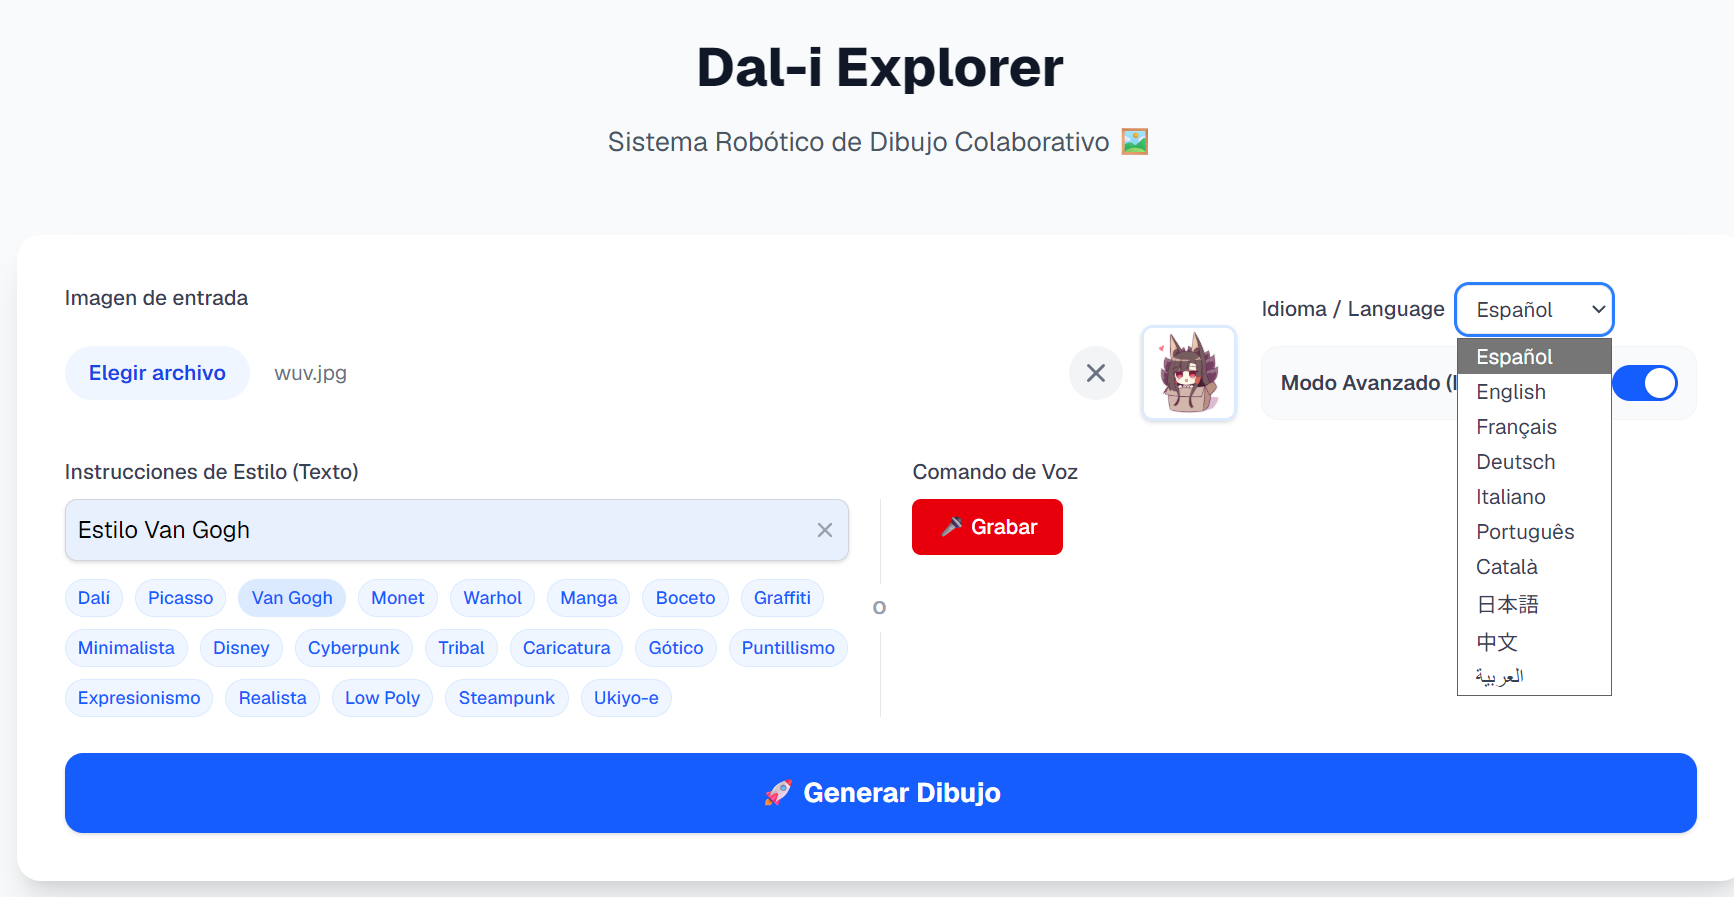
\includegraphics[width=\linewidth]{app_screenshot.png}
  \caption{Interfície principal de Dal-i amb el selector d'idioma desplegat.}
  \label{fig:app}
\end{figure}

La \cref{fig:app} mostra l'estat de la interfície amb una imatge seleccionada, un estil introduït per text i el selector d'idioma desplegat, mostrant els 10 idiomes disponibles.

\section{Arquitectura del Sistema}
\label{sec:arquitectura}

\subsection{Visió general}

El sistema Dal-i segueix una arquitectura de microserveis \textit{cloud-native} desplegada completament sobre Google Cloud Platform (GCP). La decisió de separar les operacions lleugeres (historial, càrrega d'imatges, parla i traducció) en Cloud Functions~\cite{cloudfunctions} independents, mantenint el pipeline de visió computacionalment intens en un servei Cloud Run~\cite{cloudrun} dedicat, permet escalar cada component de forma independent i reduir costos quan el sistema no està en ús.

La \cref{fig:arquitectura} mostra el diagrama d'arquitectura del sistema:

\begin{figure}[H]
\centering
\begin{tikzpicture}[
    node distance=0.8cm and 1.4cm,
    box/.style={draw, rounded corners=4pt, minimum width=3.8cm,
                minimum height=0.9cm, align=center, font=\small\sffamily,
                fill=dalblue!8, draw=dalblue!40},
    storage/.style={box, fill=gray!10, draw=gray!40},
    arr/.style={-{Stealth[length=5pt]}, thick, color=dalblue!70},
    lbl/.style={font=\scriptsize\sffamily\color{gray}, midway},
  ]

  \node[font=\scriptsize\sffamily\color{gray!80}, align=center] (auth)
    {\faLock\; Firebase Anonymous Auth};

  \node[box, below=0.3cm of auth] (fe)
    {\faDesktop\\[2pt]\textbf{Frontend}\\{\scriptsize Next.js · React · TS}};

  \node[box, below=1.0cm of fe] (cf)
    {\faCloud\\[2pt]\textbf{Cloud Functions}\\
     {\scriptsize history · upload · speech}};

  \node[box, right=2.2cm of cf] (cr)
    {\faCog\\[2pt]\textbf{Cloud Run}\\{\scriptsize FastAPI · Vision}};

  \node[storage, below=1.0cm of cf] (ai)
    {\faBrain\\[2pt]\textbf{Vertex AI · Gemini}\\
     {\scriptsize Speech · TTS · Translate}};

  \node[storage, below=1.0cm of cr] (fs)
    {\faDatabase\\[2pt]\textbf{Firestore + GCS}};

  \draw[arr] (fe)  -- node[lbl, left]{REST} (cf);
  \draw[arr] (cf)  -- node[lbl, above]{REST} (cr);
  \draw[arr] (cf)  -- (ai);
  \draw[arr] (cr)  -- (fs);
  \draw[arr] (cr.south) to[out=-120, in=30] (ai.east);

\end{tikzpicture}
\caption{Diagrama d'arquitectura del sistema Dal-i sobre Google Cloud Platform.}
\label{fig:arquitectura}
\end{figure}

\subsection{Frontend}

El frontend és una aplicació \textbf{Next.js 16}~\cite{nextjs} (React 19~\cite{react}, TypeScript, Tailwind CSS 4~\cite{tailwind}) compilada com a exportació estàtica (\texttt{output: "export"}). El bundle resultant es serveix directament des del contenidor Cloud Run, sense necessitat d'un servidor de renderització independent.

La comunicació amb el backend es centralitza al mòdul \texttt{app/lib/api.ts}, que s'encarrega d'injectar automàticament el token de Firebase Anonymous Auth~\cite{firebase} a totes les peticions com a capçalera \texttt{Authorization: Bearer <token>}. L'autenticació és completament transparent per a l'usuari: el SDK de Firebase crida \texttt{signInAnonymously()} en el primer muntatge del component i retorna un UID estable i persistent per al navegador.

\subsection{Cloud Run — Backend de Visió}

El servei Cloud Run~\cite{cloudrun} (\texttt{dal-i-api}, regió \texttt{europe-west1}) és un contenidor Docker que executa una API REST amb FastAPI~\cite{fastapi}. Conté el pipeline de processament d'imatges (computacionalment intens) i serveix els endpoints principals:

\begin{itemize}
  \item \texttt{GET /health}: comprovació d'estat del servei.
  \item \texttt{POST /process}: pipeline complet per a selecció d'estil per botons.
  \item \texttt{POST /process/voice}: pipeline per a entrada de veu (compatible amb Raspberry Pi).
  \item \texttt{POST /process/text}: pipeline per a entrada de text (compatible amb Raspberry Pi).
\end{itemize}

Els endpoints \texttt{/process} requereixen un token de Firebase vàlid (o retornen \texttt{uid="device"} per a clients sense autenticació, com la Raspberry Pi). Tots els endpoints estan protegits per un limitador de velocitat en memòria (\textit{sliding window}, 20 peticions/minut per IP).

El Dockerfile és multi-etapa: la primera etapa compila el frontend amb Node.js 20, i la segona copia el bundle estàtic i el codi Python al contenidor final basat en Python 3.12 slim.

\subsection{Cloud Functions}

Tres Cloud Functions~\cite{cloudfunctions} de 2a generació gestionen les operacions lleugeres:

\subsubsection*{history}
Gestiona el CRUD de l'historial de generacions per usuari sobre Firestore~\cite{firestore}. Suporta:
\begin{itemize}
  \item \texttt{GET}: llistat paginat (cursor basat en \texttt{start\_after(snapshot)}, 12 elements per pàgina).
  \item \texttt{DELETE ?id=\{docId\}}: esborra un element de Firestore \textbf{i} les imatges associades de Cloud Storage~\cite{gcs}.
  \item \texttt{DELETE ?deleteAll=true}: esborra tots els elements de l'usuari en lots de fins a 500 (límit de batch de Firestore) i els blobs de GCS en cascada.
\end{itemize}

\subsubsection*{upload}
Accepta una imatge per POST (\texttt{multipart/form-data}), la valida (màxim 10 MB, MIME \texttt{image/*}) i la puja al bucket \texttt{dal-i-bucket} de Cloud Storage~\cite{gcs} amb accés públic. Retorna l'URL pública i el nom del fitxer.

\subsubsection*{speech}
Agrupa tres operacions de parla i traducció en un sol endpoint amb paràmetre \texttt{?action=}:
\begin{itemize}
  \item \texttt{transcribe}: rep un fitxer d'àudio WebM/Opus, el transcriu amb Cloud Speech-to-Text~\cite{stt} en l'idioma seleccionat, tradueix la transcripció a l'anglès (Cloud Translation~\cite{translate}), i extreu l'estil artístic.
  \item \texttt{tts}: rep text en anglès i un codi d'idioma destí, tradueix el text a l'idioma de l'usuari, genera l'àudio MP3 amb Cloud TTS~\cite{tts} (veus Journey o WaveNet) i el retorna en base64.
  \item \texttt{translate}: traducció de text simple entre qualsevol parell d'idiomes suportats.
\end{itemize}

Totes les Cloud Functions verifiquen el token de Firebase amb
\code{firebase\_admin.auth().verify\_id\_token(token)}
i afegeixen les capçaleres CORS necessàries per permetre crides des del domini de Cloud Run.

\subsection{Emmagatzematge i Bases de Dades}

\textbf{Cloud Storage}~\cite{gcs} (\code{dal-i-bucket}) emmagatzema les imatges d'entrada (\code{images/}), les imatges transformades per Gemini i els resultats JSON amb les coordenades (\code{results/}). Tots els blobs es fan públics en el moment de la pujada.

\textbf{Firestore}~\cite{firestore} emmagatzema els registres de l'historial seguint la ruta \codepath{generation_history/{uid}/items/{docId}}, on \code{uid} és l'identificador anònim de Firebase. Cada registre inclou estil, URLs d'imatge, coordenades, descripció artística i marca de temps.

\subsection{Autenticació}

S'utilitza \textbf{Firebase Anonymous Authentication}~\cite{firebase}: quan un usuari accedeix a l'aplicació per primera vegada, el SDK de Firebase crea silenciosament un compte anònim i emmagatzema el token al localStorage del navegador. Aquest UID és estable entre sessions (mentre no s'esborri la memòria del navegador) i permet mantenir l'historial personal sense que l'usuari hagi de registrar-se.

El backend verifica el token a totes les peticions; per als clients de maquinari (Raspberry Pi) que no implementen Firebase Auth, el sistema admet peticions sense token i les associa a l'UID genèric \texttt{"device"}.

\section{Desenvolupament}
\label{sec:desenvolupament}

El desenvolupament del projecte s'ha organitzat en cinc fases progressives, cadascuna construint sobre l'anterior i afegint noves capacitats al sistema.

\subsection{Fase 1 — Pipeline de Visió per Computador}

El nucli del sistema és el pipeline de processament d'imatges implementat a \codepath{backend/src/vision.py}. Aquest pipeline transforma una imatge d'entrada en una llista de coordenades \code{{x, y}} que el braç robòtic pot seguir.

\subsubsection*{Detecció de contorns (Canny)}

El primer pas és la detecció de vores amb l'algoritme de Canny~\cite{canny} d'OpenCV~\cite{opencv}:

\begin{listing}[H]
\begin{minted}{python}
def detect_edges(image_bytes: bytes):
    nparr = np.frombuffer(image_bytes, np.uint8)
    img = cv2.imdecode(nparr, cv2.IMREAD_GRAYSCALE)
    img = cv2.GaussianBlur(img, (5, 5), 0)
    edges = cv2.Canny(img, threshold1=50, threshold2=150)
    contours, _ = cv2.findContours(
        edges, cv2.RETR_LIST, cv2.CHAIN_APPROX_SIMPLE
    )
    return edges, img.shape[1], img.shape[0]
\end{minted}
\caption{Detecció de vores amb Canny (\texttt{vision.py})}
\label{lst:canny}
\end{listing}

Els paràmetres de Canny (llindars 50 i 150) s'han ajustat empíricament per obtenir un bon equilibri entre la captura de detalls i el soroll (vegeu \cref{lst:canny}). Posteriorment, els contorns es simplifiquen amb \texttt{cv2.approxPolyDP} (epsilon = 0.02, àrea mínima = 20 píxels²) per reduir el nombre de punts i optimitzar el temps de dibuix del robot.

\subsubsection*{Optimització de trajectòries (TSP)}

El repte principal del robot no és dibuixar els contorns, sinó \textit{en quin ordre} i \textit{en quina direcció} fer-ho, per minimitzar el temps de desplaçament amb el bolígraf aixecat. Hem implementat una aproximació al \textit{Travelling Salesman Problem} (TSP)~\cite{tsp} en tres passes:

\begin{enumerate}
  \item \textbf{Greedy Nearest Neighbour} (\texttt{tsp\_sort\_contours}): ordena els contorns de manera voraç, triant sempre el contorn més proper al punt final del contorn anterior. Complexitat $O(n^2)$.

  \item \textbf{Optimització de direccions} (\texttt{optimize\_contour\_directions}): per a cada contorn, decideix si recórrer-lo en l'ordre original o al revés, triant la direcció que minimitza la distància des del punt final del contorn anterior.

  \item \textbf{2-opt local search} (\texttt{tsp\_two\_opt}): aplica fins a 3 passes d'intercanvi de parells de contorns per millorar la solució greedy. S'omet si hi ha més de 150 contorns per evitar temps de còmput excessius.
\end{enumerate}

\subsubsection*{Transferència d'estil (Mode Avançat)}

Quan l'usuari activa el Mode Avançat, el sistema crida \texttt{generate\_styled\_image()} que envia la imatge i el nom de l'estil a Vertex AI~\cite{vertexai} amb el model \textbf{Gemini 2.5 Flash} en mode generació d'imatges. El model retorna una versió de la imatge en l'estil artístic sol·licitat, que s'utilitza com a entrada per a Canny en lloc de la imatge original. Aquesta imatge transformada també s'emmagatzema a Cloud Storage~\cite{gcs} i es mostra a l'usuari.

\subsection{Fase 2 — Desplegament a Cloud Run}

Un cop el pipeline de visió era funcional en local, l'hem empaquetat en un contenidor Docker multi-etapa i desplegat a Cloud Run~\cite{cloudrun}:

\begin{enumerate}
  \item \textbf{Etapa 1 (Node.js 20)}: compila el frontend Next.js~\cite{nextjs} amb \texttt{npm run build}, generant l'exportació estàtica a \texttt{/frontend/out}.
  \item \textbf{Etapa 2 (Python 3.12 slim)}: instal·la les dependències Python (incloent OpenCV~\cite{opencv} i les biblioteques de GCP), copia el codi del backend i el bundle del frontend. L'arxiu \texttt{main.py} munta el directori \texttt{frontend/out} com a fitxers estàtics amb FastAPI~\cite{fastapi} \texttt{StaticFiles}.
\end{enumerate}

El desplegament automàtic s'ha configurat amb \texttt{cloudbuild.yaml}: en cada \textit{push} a \texttt{main}, Cloud Build construeix la imatge, la puja a Artifact Registry i fa un \texttt{rolling update} del servei Cloud Run sense temps d'inactivitat.

\subsection{Fase 3 — Migració a Cloud Functions i Firebase Auth}

A mesura que el sistema creixia, vam identificar que les operacions lleugeres (historial, càrrega d'imatges) no necessitaven la memòria ni les dependències pesades (OpenCV~\cite{opencv}, NumPy~\cite{numpy}) del contenidor de Cloud Run. La migració a Cloud Functions~\cite{cloudfunctions} redueix el cost de les operacions freqüents i permet escalar cada funció de forma independent.

En paral·lel, vam afegir \textbf{Firebase Anonymous Authentication}~\cite{firebase} per aïllar l'historial de cada usuari. El canvi d'esquema de Firestore~\cite{firestore} —de la col·lecció plana \codepath{generation_history/{docId}} a la subcol·lecció \codepath{generation_history/{uid}/items/{docId}}— va requerir actualitzar totes les funcions de \texttt{db.py} per acceptar el paràmetre \texttt{uid}.

La paginació de l'historial s'implementa amb el patró de cursor de Firestore: el client guarda l'ID del darrer document de la pàgina anterior i el passa com a \texttt{page\_token}; el backend fa \texttt{.start\_after(snapshot)} per obtenir la pàgina següent sense necessitat d'un \texttt{OFFSET} (que Firestore no suporta).

\subsection{Fase 4 — Suport Multilingüe}

Per donar suport a 10 idiomes, vam integrar \textbf{Cloud Translation API}~\cite{translate} a la Cloud Function \texttt{speech}. El disseny segueix el principi de \textit{traducció interna}: el sistema sempre processa en anglès internament (perquè els noms dels estils artístics estan en anglès i els models d'IA funcionen millor en aquest idioma), i tradueix automàticament tant l'entrada de l'usuari (de l'idioma seleccionat a l'anglès) com la sortida (de l'anglès a l'idioma de l'usuari).

El flux de la modalitat de veu amb Cloud Speech-to-Text~\cite{stt} i traducció és:
\[
\text{Àudio (idioma X)} \xrightarrow{\text{STT}} \text{Text (idioma X)} \xrightarrow{\text{Translate}} \text{Text (anglès)} \xrightarrow{\text{extractStyle}} \text{Estil}
\]

I el flux de la resposta amb Cloud TTS~\cite{tts}:
\[
\text{Missatge (anglès)} \xrightarrow{\text{Translate}} \text{Missatge (idioma X)} \xrightarrow{\text{TTS}} \text{Àudio (idioma X)}
\]

Per evitar crides innecessàries a l'API de traducció quan l'idioma d'origen i el destí coincideixen (anglès \arw{} anglès), s'afegeix una comprovació prèvia: si \texttt{source\_language.startswith("en")}, es retorna el text original sense traduir.

Les veus TTS s'han mapejat per a cada idioma, prioritzant les veus \textit{Journey} (més naturals) i recorrent a \textit{WaveNet} o \textit{Standard} per als idiomes sense veu Journey disponible (català, xinès, àrab).

\subsection{Fase 5 — Compatibilitat amb la Raspberry Pi}

Durant les proves d'integració, vam detectar que el braç robòtic (controlat per una Raspberry Pi) utilitzava l'endpoint \texttt{/process/voice} per enviar les imatges i l'àudio capturats localment. Quan vam migrar la parla a la Cloud Function, aquest endpoint va desaparèixer del Cloud Run, trencant la integració amb el maquinari.

La solució va ser restaurar \texttt{/process/voice} i \texttt{/process/text} al Cloud Run~\cite{cloudrun} amb una dependència d'autenticació opcional (\texttt{\_optional\_firebase\_token}): si la petició no porta cap token, el sistema continua amb l'\texttt{uid} genèric \texttt{"device"} en comptes de retornar un error 401. Això permet que la Raspberry Pi operi sense implementar Firebase Auth~\cite{firebase}.

\section{Tecnologies Utilitzades}
\label{sec:tecnologies}

\subsection{Serveis Cloud (Google Cloud Platform)}

La \cref{tab:cloud} recull tots els serveis GCP utilitzats al projecte.

\begin{table}[H]
\centering
\caption{Serveis GCP utilitzats al projecte Dal-i.}
\label{tab:cloud}
\begin{tabularx}{\linewidth}{p{4.2cm}X}
\toprule
\textbf{Servei} & \textbf{Ús en el projecte} \\
\midrule
Cloud Run~\cite{cloudrun} & Backend FastAPI + frontend estàtic. Executa el pipeline de visió, els endpoints \texttt{/process*} i serveix el bundle Next.js. Regió: \texttt{europe-west1}. \\[4pt]
Cloud Functions~\cite{cloudfunctions} & Tres funcions lleugeres: \texttt{history} (CRUD Firestore), \texttt{upload} (pujada a GCS) i \texttt{speech} (STT, TTS, traducció). Regió: \texttt{us-central1}. \\[4pt]
Vertex AI / Gemini~\cite{vertexai} & Transferència d'estil visual image-to-image en el Mode Avançat. Model: \texttt{gemini-2.5-flash}. Crida des de Cloud Run. \\[4pt]
Cloud Speech-to-Text~\cite{stt} & Transcripció d'àudio WebM/Opus a text. Suporta multiidioma amb \texttt{alternative\_language\_codes}. Crida des de la CF \texttt{speech}. \\[4pt]
Cloud Text-to-Speech~\cite{tts} & Síntesi de veu (MP3) a partir de text. Veus Journey i WaveNet per a 10 idiomes. Crida des de la CF \texttt{speech}. \\[4pt]
Cloud Translation API~\cite{translate} & Traducció automàtica de text entre qualsevol parell dels 10 idiomes suportats. Crida des de la CF \texttt{speech}. \\[4pt]
Cloud Storage~\cite{gcs} & Emmagatzematge d'imatges d'entrada, imatges estilitzades i resultats JSON. Bucket: \texttt{dal-i-bucket}. \\[4pt]
Firestore~\cite{firestore} & Base de dades documental per a l'historial per usuari. Col·lecció: \codepath{generation_history/{uid}/items}. \\[4pt]
Firebase Auth~\cite{firebase} & Autenticació anònima del costat del client. UID persistent per navegador sense registre de l'usuari. \\[4pt]
Cloud Build & CI/CD per a Cloud Run: construeix la imatge Docker, la puja a Artifact Registry i desplega el servei. \\[4pt]
Artifact Registry & Registre privat d'imatges Docker del projecte. \\
\bottomrule
\end{tabularx}
\end{table}

\subsection{Tecnologies No-Cloud}

La \cref{tab:nocloud} recull les tecnologies i biblioteques no-cloud del projecte.

\begin{table}[H]
\centering
\caption{Tecnologies no-cloud utilitzades al projecte.}
\label{tab:nocloud}
\begin{tabularx}{\linewidth}{p{4.2cm}lX}
\toprule
\textbf{Tecnologia} & \textbf{Versió} & \textbf{Ús en el projecte} \\
\midrule
Python & 3.12 & Llenguatge principal del backend i les Cloud Functions. \\[3pt]
FastAPI~\cite{fastapi} & 0.110 & Framework REST del backend; gestió de rutes, validació Pydantic i middlewares CORS. \\[3pt]
OpenCV~\cite{opencv} & 4.9 & Detecció de vores (Canny), extracció de contorns (\texttt{findContours}) i simplificació (\texttt{approxPolyDP}). \\[3pt]
NumPy~\cite{numpy} & 1.26 & Operacions matricials en el processament d'imatges i càlcul de distàncies per a l'algoritme TSP. \\[3pt]
Pillow & 10.4 & Redimensionament i conversió de format de les imatges d'entrada. \\[3pt]
firebase-admin & 6.5 & Verificació de tokens Firebase al backend (Cloud Run i Cloud Functions). \\[3pt]
functions-framework & 3.8 & Execució de Cloud Functions Python tant en local com en producció. \\[3pt]
httpx & 0.27 & Client HTTP asíncron per a crides entre serveis interns. \\[3pt]
Next.js~\cite{nextjs} & 16.2 & Framework React per al frontend, compilat com a exportació estàtica. \\[3pt]
React~\cite{react} & 19.2 & Biblioteca d'interfície d'usuari amb hooks per a la gestió d'estat. \\[3pt]
TypeScript & 5.x & Tipat estàtic del codi frontend per evitar errors en temps d'execució. \\[3pt]
Tailwind CSS~\cite{tailwind} & 4.x & Estils utilitaris per a la interfície d'usuari responsiva. \\[3pt]
Firebase SDK (JS) & 10.x & Autenticació anònima i obtenció de tokens al costat del client (navegador). \\[3pt]
Docker & — & Contenidor multi-etapa per empaquetar backend Python i frontend estàtic. \\[3pt]
pnpm & 11.2 & Gestor de paquets Node.js amb gestió eficient del workspace. \\[3pt]
pytest & 8.2 & Framework de tests unitaris per al backend Python. \\
\bottomrule
\end{tabularx}
\end{table}

\subsection{Organització del Codi Font}

El repositori~\cite{github} s'organitza de la manera següent per reflectir clarament la separació entre Cloud Run i Cloud Functions:

\begin{listing}[H]
\begin{minted}[linenos=false]{text}
SM-MiniProjecte2026/
├── backend/           # Cloud Run: FastAPI + pipeline de visió
│   └── src/
│       ├── main.py    # Endpoints /process, /process/voice, /process/text
│       ├── vision.py  # Canny, TSP, Gemini
│       ├── speech.py  # Wrapper Cloud Speech/TTS
│       ├── db.py      # CRUD Firestore per usuari
│       └── storage.py # Helpers Cloud Storage
├── cloudfunctions/    # Cloud Functions: operacions lleugeres
│   ├── history/       # GET/DELETE historial
│   ├── upload/        # POST pujada d'imatge
│   └── speech/        # Transcripció, TTS i traducció
└── frontend/          # Next.js 16 - interfície web
    └── app/
        └── lib/
            ├── firebase.ts       # Init Firebase + signInAnon
            ├── api.ts            # Client API centralitzat
            └── styleExtractor.ts # extractStyle() en TypeScript
\end{minted}
\caption{Estructura del repositori (simplificada).}
\label{lst:repo}
\end{listing}

\section{Problemes i Solucions}
\label{sec:problemes}

Durant el desenvolupament del projecte hem trobat diversos problemes tècnics. En aquest apartat documentem els més significatius, la causa arrel i la solució adoptada.

\subsection*{Problema 1 — Firebase \textit{auth/invalid-api-key} durant el build de producció}

\textbf{Símptoma.} El build de Docker fallava amb l'error \texttt{Firebase: Error (auth/invalid-api-key)} durant la fase de compilació del frontend Next.js. El build resultava en un codi d'error 1.

\textbf{Causa.} Next.js realitza un pre-render estàtic de totes les pàgines durant el build (\textit{Static Site Generation}). El mòdul \texttt{firebase.ts} cridava \texttt{initializeApp()} a nivell de mòdul (fora de qualsevol funció), de manera que s'executava durant el pre-render. En aquell moment, les variables d'entorn \texttt{NEXT\_PUBLIC\_FIREBASE\_*} no estaven disponibles (el fitxer \texttt{.env} s'exclou del context de Docker per seguretat), i Firebase rebria una clau d'API buida.

\textbf{Solució.} Es va reimplementar \texttt{firebase.ts} amb \textbf{inicialització diferida} (\textit{lazy initialization}): \texttt{initializeApp()} s'executa dins d'una funció getter (\texttt{getFirebaseAuth()}) que es crida per primera vegada des d'un \texttt{useEffect} del navegador, mai durant el pre-render. A més, es va afegir \texttt{auth.authStateReady()} per esperar que Firebase restauri l'estat d'autenticació del localStorage abans de fer cap petició autenticada. Es va crear el fitxer \texttt{frontend/.env.production} (comès al repositori, ja que conté valors públics) amb les variables necessàries.

\subsection*{Problema 2 — Variable \textit{\$SHORT\_SHA} buida en desplegament manual}

\textbf{Símptoma.} En executar \texttt{gcloud builds submit} manualment des de la línia de comandes, el build fallava amb l'error \textit{«invalid image name: could not parse reference»} perquè el nom de la imatge Docker incloïa una etiqueta buida (\texttt{:}).

\textbf{Causa.} El fitxer \code{cloudbuild.yaml} utilitza la variable \code{\$SHORT\_SHA} (hash curt del commit git) per etiquetar les imatges Docker. Aquesta variable s'injecta automàticament quan Cloud Build s'activa des d'un \textit{trigger} de repositori, però no s'injecta quan es fa un \code{gcloud builds submit} manual.

\textbf{Solució.} Passar la substitució explícitament en cada execució manual:
\begin{minted}[linenos=false]{bash}
gcloud builds submit --config cloudbuild.yaml \
  --substitutions=SHORT_SHA=$(git rev-parse --short HEAD)
\end{minted}

\subsection*{Problema 3 — Error 403 en el desplegament de Cloud Functions}

\textbf{Símptoma.} El primer desplegament d'una Cloud Function fallava indicant que el service agent no tenia els permisos \code{artifactregistry.repositories.list} i \code{artifactregistry.repositories.get}.

\textbf{Causa.} Cloud Functions de 2a generació utilitza Artifact Registry per emmagatzemar els contenidors de les funcions. El compte de servei del servei Cloud Functions (\texttt{service-PROJECT\_NUMBER@gcf-admin-robot.iam.gserviceaccount.com}) no tenia els permisos necessaris sobre Artifact Registry.

\textbf{Solució.} Afegir el rol \texttt{roles/artifactregistry.reader} al compte de servei:
\begin{minted}[linenos=false]{bash}
gcloud projects add-iam-policy-binding PROJECT_ID \
  --member="serviceAccount:service-NUMBER@gcf-admin-robot.iam.gserviceaccount.com" \
  --role="roles/artifactregistry.reader"
\end{minted}

\subsection*{Problema 4 — Botó de generació desactivat en producció}

\textbf{Símptoma.} Desplegada l'aplicació a Cloud Run, el botó «Generar Dibujo» apareixia sempre en gris desactivat. No es produïa cap missatge d'error visible.

\textbf{Causa.} El botó es desactiva mentre \texttt{uid === null}, és a dir, mentre Firebase no hagi completat el login anònim. La crida a \texttt{signInAnonymously()} fallava silenciosament perquè el domini de Cloud Run (\texttt{dal-i-api-y55wqasb6a-ew.a.run.app}) no estava a la llista de dominis autoritzats de Firebase Authentication.

\textbf{Solució en dues passes.}
\begin{enumerate}
  \item Afegir el domini al panell de Firebase Console \arw{} Authentication \arw{} Settings \arw{} Authorized domains.
  \item Modificar el bloc \texttt{catch} de \texttt{signInAnon()} per mostrar l'error a la interfície (en comptes de silenciar-lo), facilitant el diagnòstic futur.
\end{enumerate}

\subsection*{Problema 5 — \texttt{auth/admin-restricted-operation}}

\textbf{Símptoma.} Després de solucionar el problema anterior, l'error canviava a \texttt{Firebase: Error (auth/admin-restricted-operation)}.

\textbf{Causa.} Tot i tenir el domini autoritzat, el proveïdor d'autenticació anònima no estava habilitat al projecte Firebase.

\textbf{Solució.} Activar el proveïdor anònim a Firebase Console \arw{} Authentication \arw{} Sign-in method \arw{} Anonymous \arw{} Enable.

\subsection*{Problema 6 — La Raspberry Pi rebia 404 a \textit{/process/voice}}

\textbf{Símptoma.} Després de la migració de la parla a Cloud Functions, la Raspberry Pi deixava de rebre coordenades. La petició retornava codi 404.

\textbf{Causa.} Durant la migració a Cloud Functions, els endpoints \texttt{/process/voice} i \texttt{/process/text} es van eliminar del Cloud Run perquè el frontend web ja no els necessitava (orquestraria les crides a la CF directament). Però la Raspberry Pi continuava cridant l'endpoint original del Cloud Run.

\textbf{Solució.} Restaurar \texttt{/process/voice} i \texttt{/process/text} al Cloud Run, afegint una dependència d'autenticació opcional (\texttt{\_optional\_firebase\_token}) que retorna \texttt{uid="device"} quan no hi ha token, en lloc de retornar error 401. D'aquesta manera els dos clients (navegador i Pi) coexisteixen sense canvis al codi de la Pi.

\subsection*{Problema 7 — Context de Docker de 364 MB}

\textbf{Símptoma.} Cada \texttt{gcloud builds submit} pujava 364 MB de context al núvol, alentint el procés i consumint quota de Cloud Storage innecessàriament.

\textbf{Causa.} El directori de treball incloïa \texttt{frontend/node\_modules/} (uns 300 MB) en el context de build, tot i existir un fitxer \texttt{.gcloudignore}.

\textbf{Solució.} Verificar i completar el fitxer \texttt{.gcloudignore} per excloure explícitament \texttt{node\_modules/}, \texttt{frontend/.next/}, \texttt{frontend/out/}, \texttt{backend/.venv/} i els directoris \texttt{docs/}.

\section{Resultats}
\label{sec:resultats}

\subsection{Sistema en Producció}

El sistema Dal-i es troba desplegat i accessible públicament a:
\begin{center}
  \url{https://dal-i-api-y55wqasb6a-ew.a.run.app}
\end{center}

L'aplicació és funcional en els tres modes d'entrada (selecció, text i veu), amb suport per a 10 idiomes i el Mode Avançat activable. Les Cloud Functions responen de manera independent i el historial per usuari es manté entre sessions.

\subsection{Pipeline de Visió}

El pipeline complet (sense Mode Avançat) processa una imatge típica de 768×768 píxels en \textbf{2--5 segons}, depenent del nombre de contorns detectats. Amb el Mode Avançat activat (crida a Gemini), el temps total augmenta fins als \textbf{10--20 segons} segons la complexitat de la imatge i la disponibilitat del model.

El sistema genera típicament entre \textbf{50 i 500 traços} per imatge, cadascun representat com una seqüència de punts \texttt{\{x, y\}}. L'optimització TSP (Greedy + 2-opt) redueix el desplaçament en buit del robot entre un 20\% i un 40\% respecte a un ordre aleatori dels contorns.

\subsection{Exemples de Resultats}

La \cref{fig:akagi} i la \cref{fig:koharu} mostren exemples de processament amb el sistema. Cada parell mostra la imatge d'entrada (esquerra) i el resultat del sistema (dreta), que representa els traços que el robot executarà.

\begin{figure}[H]
  \centering
  \begin{subfigure}[t]{0.47\linewidth}
    \centering
    
\includegraphics[width=\linewidth]{akagi pre.png}
    \caption{Imatge d'entrada (Akagi)}
  \end{subfigure}
  \hfill
  \begin{subfigure}[t]{0.47\linewidth}
    \centering
    
\includegraphics[width=\linewidth]{akagi.png}
    \caption{Trazos SVG generats (sense Mode Avançat)}
  \end{subfigure}
  \caption{Personatge Akagi — processament bàsic, sense IA generativa: només detecció de contorns i vectors SVG.}
  \label{fig:akagi}
\end{figure}

\begin{figure}[H]
  \centering
  \begin{subfigure}[t]{0.47\linewidth}
    \centering
    
\includegraphics[width=\linewidth]{koharu pre.jpg}
    \caption{Imatge d'entrada (Koharu)}
  \end{subfigure}
  \hfill
  \begin{subfigure}[t]{0.47\linewidth}
    \centering
    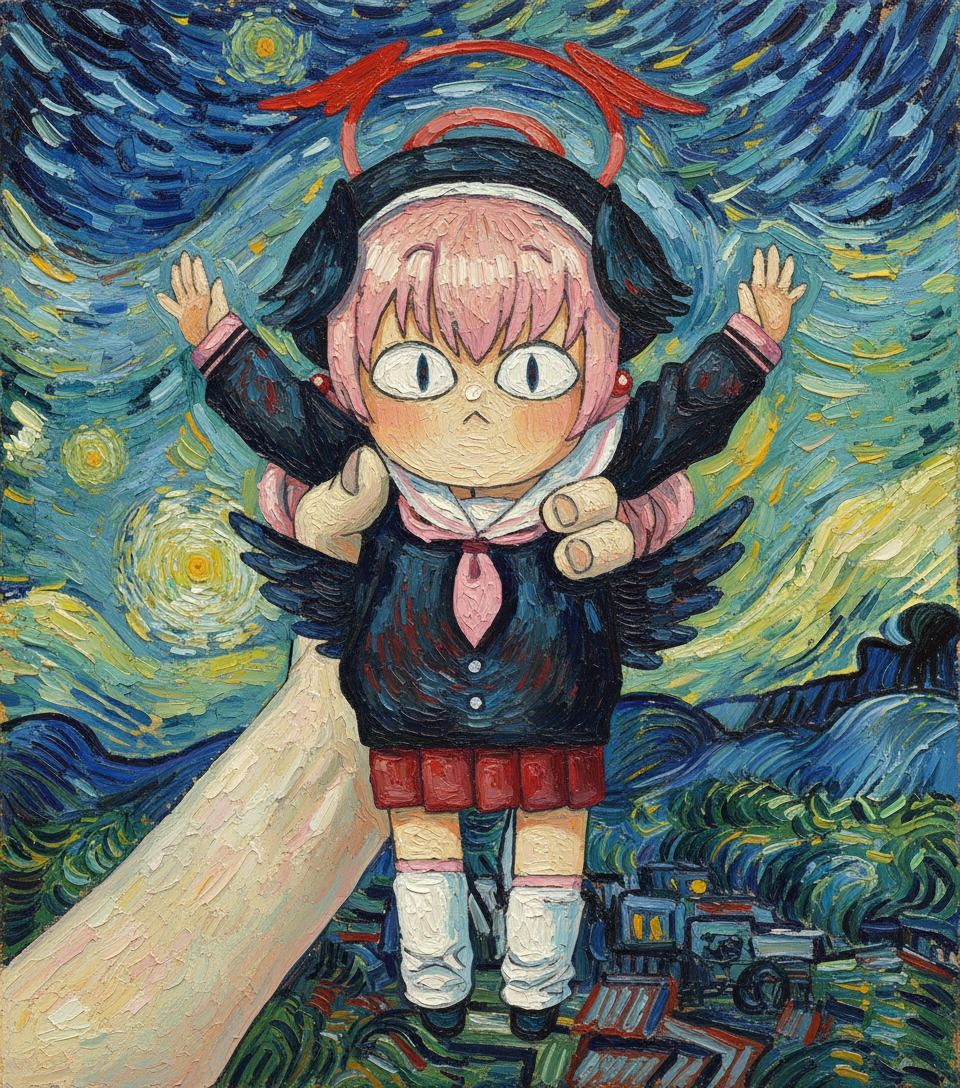
\includegraphics[width=\linewidth]{koharu.jpeg}
    \caption{Resultat amb Mode Avançat (estil Van Gogh)}
  \end{subfigure}
  \caption{Personatge Koharu — Mode Avançat activat: Gemini 2.5 Flash aplica l'estil Van Gogh abans de la detecció de contorns.}
  \label{fig:koharu}
\end{figure}

\subsection{Tests}

El projecte inclou una suite de tests unitaris per al backend Python, situada a \texttt{backend/tests/}. Els tests cobreixen els endpoints principals del Cloud Run (\texttt{/health}, \texttt{/process}, \texttt{/process/voice}, \texttt{/process/text}) i els mòduls de visió, parla i emmagatzematge. En el moment de tancament del projecte, \textbf{39 tests passen} sense errors amb pytest.

La dependència d'autenticació Firebase s'injecta com a \textit{mock} als tests mitjançant \texttt{app.dependency\_overrides[\_verify\_firebase\_token] = lambda: "test-uid"}, de manera que els tests no necessiten un token real de Firebase.

\subsection{Infraestructura Desplegada}

La \cref{tab:deployed} recull tots els recursos GCP actius en el moment de tancament del projecte.

\begin{table}[H]
\centering
\caption{Resum dels recursos GCP desplegats.}
\label{tab:deployed}
\begin{tabular}{@{}llll@{}}
\toprule
\textbf{Recurs} & \textbf{Nom} & \textbf{Regió} & \textbf{Estat} \\
\midrule
Cloud Run & \texttt{dal-i-api} & \texttt{europe-west1} & Actiu \\
Cloud Function & \texttt{history} & \texttt{us-central1} & Actiu \\
Cloud Function & \texttt{upload} & \texttt{us-central1} & Actiu \\
Cloud Function & \texttt{speech} & \texttt{us-central1} & Actiu \\
Cloud Storage & \texttt{dal-i-bucket} & Multirègió & Actiu \\
Firestore & — & \texttt{us-central1} & Actiu \\
Firebase Auth & — & Global & Actiu \\
\bottomrule
\end{tabular}
\end{table}

\section{Conclusions i Treball Futur}
\label{sec:conclusions}

\subsection{Conclusions}

El projecte Dal-i ha assolit tots els objectius plantejats inicialment. S'ha dissenyat i implementat un sistema complet que cobreix des de la interfície d'usuari fins al maquinari robòtic, passant per un pipeline de visió per computador, models d'IA generativa i una infraestructura \textit{cloud-native} escalable.

Les conclusions principals del projecte són les següents:

\begin{description}
  \item[Arquitectura de microserveis.] La separació entre Cloud Run (pipeline de visió, computacionalment intens) i Cloud Functions (operacions lleugeres de dades i parla) ha demostrat ser una decisió encertada. Permet escalar cada component de forma independent i reduir el cost quan el sistema està en repòs, ja que les Cloud Functions no generen cost si no hi ha invocacions.

  \item[Firebase Anonymous Auth.] L'autenticació anònima ha resultat ser una solució elegant per oferir un historial persistent per sessió sense forçar l'usuari a registrar-se. L'UID estable permet associar les dades a un navegador concret sense necessitar cap formulari de registre.

  \item[Traducció automàtica interna.] Processar sempre en anglès internament i traduir les entrades i sortides automàticament ha simplificat enormement el codi de processament d'estils, que no necessita conèixer cap idioma específic. El resultat és un sistema multilingüe robust amb un sobrecost de latència mínim.

  \item[Optimització TSP per a robòtica.] L'aplicació de tècniques d'optimització de rutes (Greedy Nearest Neighbour + 2-opt) al problema d'ordenació de contorns per al robot ha tingut un impacte positiu mesurable en el temps de dibuix. Aquesta connexió entre algorísmica clàssica i robòtica ha estat un dels aspectes més enriquidors del projecte.

  \item[Integració de maquinari.] La coexistència de clients diversos (navegador web amb Firebase Auth i Raspberry Pi sense autenticació) s'ha resolt de manera neta amb la dependència d'autenticació opcional, sense duplicar cap lògica de negoci.
\end{description}

\subsection{Aprenentatges}

El projecte ha permès adquirir experiència pràctica en:

\begin{itemize}
  \item Desplegament de contenidors Docker multi-etapa a Google Cloud Run.
  \item Implementació i desplegament de Cloud Functions de 2a generació amb Python.
  \item Configuració d'autenticació Firebase en aplicacions web estàtiques (Next.js static export).
  \item Integració de múltiples APIs de GCP (Speech-to-Text, TTS, Translation, Vertex AI) en un sol sistema coherent.
  \item Algorísmica aplicada (TSP) en un context de robòtica real.
  \item Gestió de problemes de CORS, IAM i dominis autoritzats en entorns de producció.
\end{itemize}

\subsection{Treball Futur}

Com a línies de treball futur, proposem les extensions següents:

\begin{enumerate}
  \item \textbf{Generació de vídeo del procés de dibuix.} Capturar la trajectòria del robot en temps real i generar un vídeo time-lapse del dibuix, que es podria compartir directament des de la interfície.

  \item \textbf{Col·laboració en temps real.} Permetre que múltiples usuaris contribueixin a un mateix dibuix simultàniament, amb sincronització via WebSockets o Firebase Realtime Database.

  \item \textbf{Ampliació d'estils artístics.} Incorporar un mecanisme de \textit{fine-tuning} de Gemini per afegir nous estils artístics de manera dinàmica, sense canvis al codi.

  \item \textbf{Dashboard d'administració.} Crear un panell de control per monitoritzar l'ús del sistema, els costos de GCP i les estadístiques de dibuixos generats.

  \item \textbf{Optimització del pipeline amb GPU.} Explorar l'execució del pipeline de visió en una instància amb GPU a Cloud Run per accelerar el processament de Mode Avançat.

  \item \textbf{Exportació en formats estàndard.} Permetre descarregar les trajectòries generades en formats industrials com G-code o SVG optimitzat, compatibles amb una gamma més àmplia de màquines CNC i plotters.
\end{enumerate}


\newpage
\nocite{*}
\printbibliography[heading=bibintoc, title={Referències}]

\end{document}
